\documentclass{article}

\usepackage{tikz}

\usetikzlibrary{positioning,calc}

\begin{document}
\begin{figure}[!htb]
\begin{center}
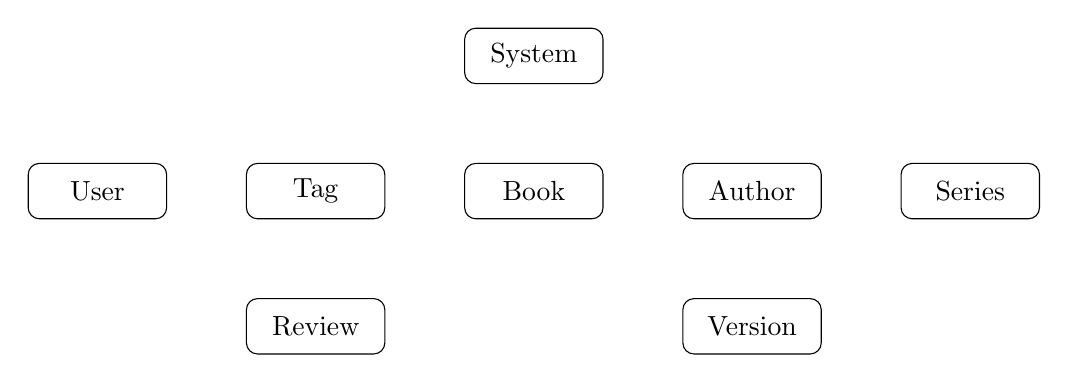
\begin{tikzpicture}
[auto,
class/.style={rectangle,draw=black,align=center,minimum height=2em, minimum width=5em, rounded corners}
]

\node [class] (system) {System};

\node [class, below left = of system] (tag) {Tag};
\node [class, left = of tag] (user) {User};
\node [class, below right = of system] (author) {Author};
\node [class, right = of author] (series) {Series};

\node [class, below = of system] (book) {Book};
\node [class, below right = of book] (versions) {Version};
\node [class, below left = of book] (reviews) {Review};

\end{tikzpicture}
\end{center}
\end{figure}
\end{document}